
\begin{frame}[c]{Le motivazioni alla base di questo lavoro}

In uno \textit{smartphone}, come in molti ambienti embedded, le risorse sono limitate. Utilizzarle correttamente non è solo un esercizio di stile o una azione eticamente corretta (nei confronti dell'utente, a cui le risorse ``appartengono"), ma anche un modo per rendere il sistema efficiente.

\vspace{0.5cm}
Un sistema che è in grado di fornire una migliore \textit{user experience} (grazie all'efficienza) gratifica l'utente nella scelta della applicazione.

\end{frame}

\begin{frame}[c]{Roadmap}

\begin{itemize}
\item I Terremoti
\item Il progetto SeismoCloud
\item Ottimizzazione energetica
\item Ottimizzazione della rete
\item Ottimizzazione in fase di sviluppo
\item Sviluppi futuri
\end{itemize}

\end{frame}

\section{I terremoti}

\begin{frame}[c]{Origine}
\begin{center}
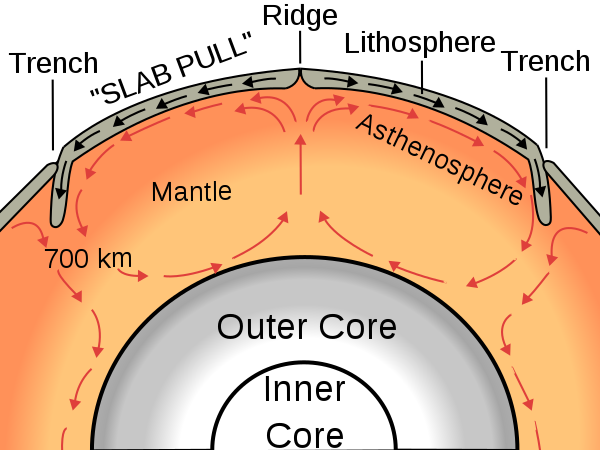
\includegraphics[scale=0.35]{introduzione/oceanic_spreading}
\end{center}
\end{frame}

\begin{frame}[c]{Le faglie italiane}
\begin{center}
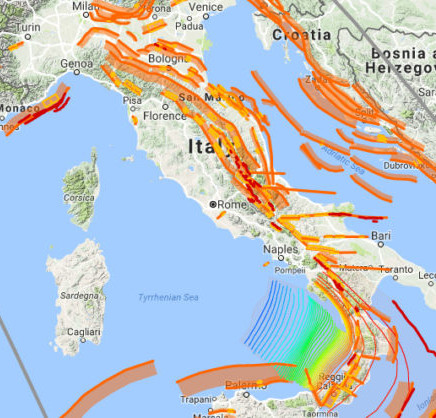
\includegraphics[scale=0.4]{introduzione/mappa_faglie_italiane2}
\end{center}
\end{frame}

\begin{frame}[c]{Previsione, prevenzione e gestione}

Nonostante i progressi nella ricerca, \textbf{i terremoti non sono (ancora) previdibili}.

\vspace{0.5cm}
Dobbiamo quindi affidarci alla \textbf{prevenzione} e alla \textbf{gestione dell'emergenza}.

\vspace{0.5cm}
Mentre la rete IV dell'Istituto Nazionale di Geofisica e Vulcanologia è utile in fase di prevenzione (grazie ai dati accumulati e studiati nel tempo), il progetto \textbf{SeismoCloud} si posiziona tra il momento in cui il terremoto si presenta nell'epicentro, ed il momento in cui colpisce le zone circostanti.

\end{frame}

\section{SeismoCloud}

\begin{frame}[c]{SeismoCloud}

\textbf{SeismoCloud} è un progetto di \textit{early warning} mediante \textit{crowdsourcing}.

\vspace{0.5cm}
Grazie ad una rete di sensori fissi e mobili, il sistema acquisisce i dati sulle possibili scosse, li analizza ed eventualmente genera una notifica.

\vspace{0.5cm}
L'obiettivo di SeismoCloud è quello di \textbf{anticipare la scossa di terremoto}, grazie alla differente velocità delle onde radio e delle scosse di terremoto.

\end{frame}

\begin{frame}[c]{Architettura}
\begin{center}
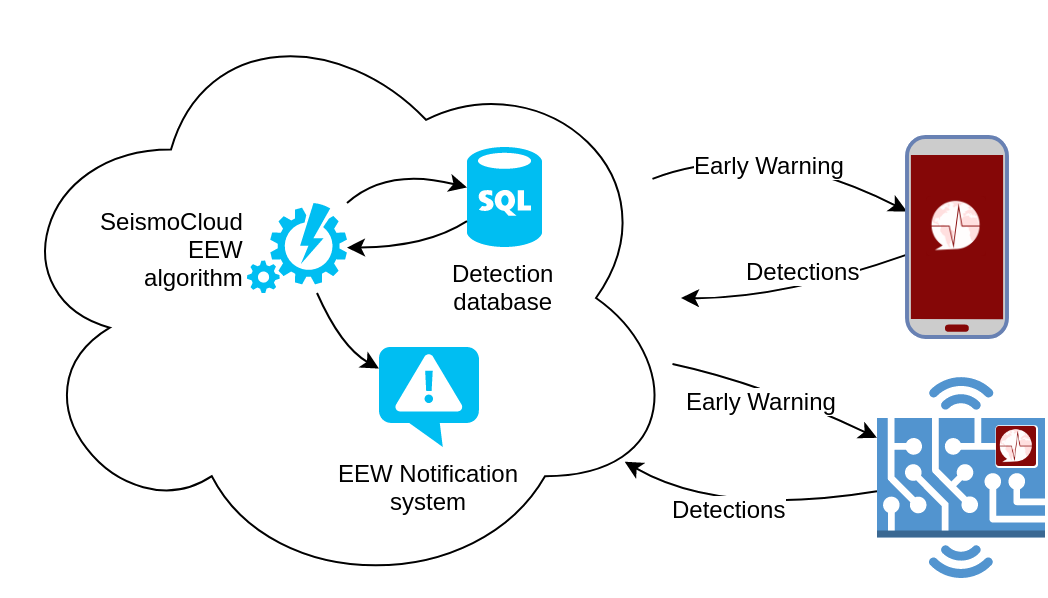
\includegraphics[scale=0.3]{introduzione/SeismoCloud_arch}
\end{center}
\end{frame}

\begin{frame}[c]{I telefoni come sensori}
\begin{center}
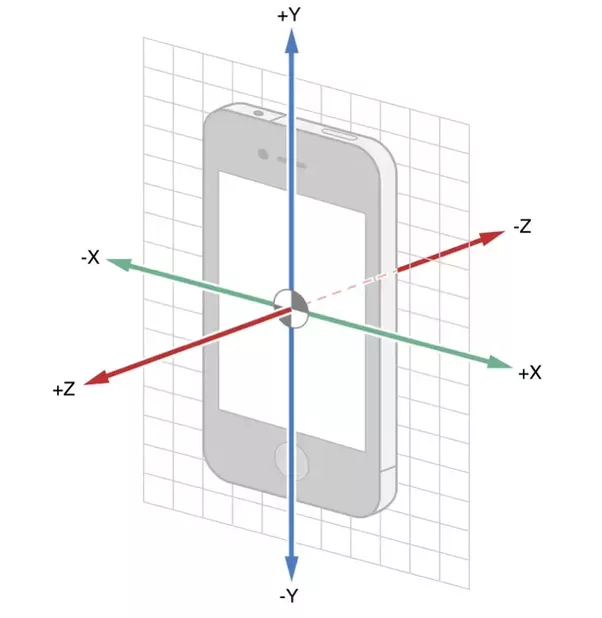
\includegraphics[scale=0.3]{introduzione/smartphone_axes}
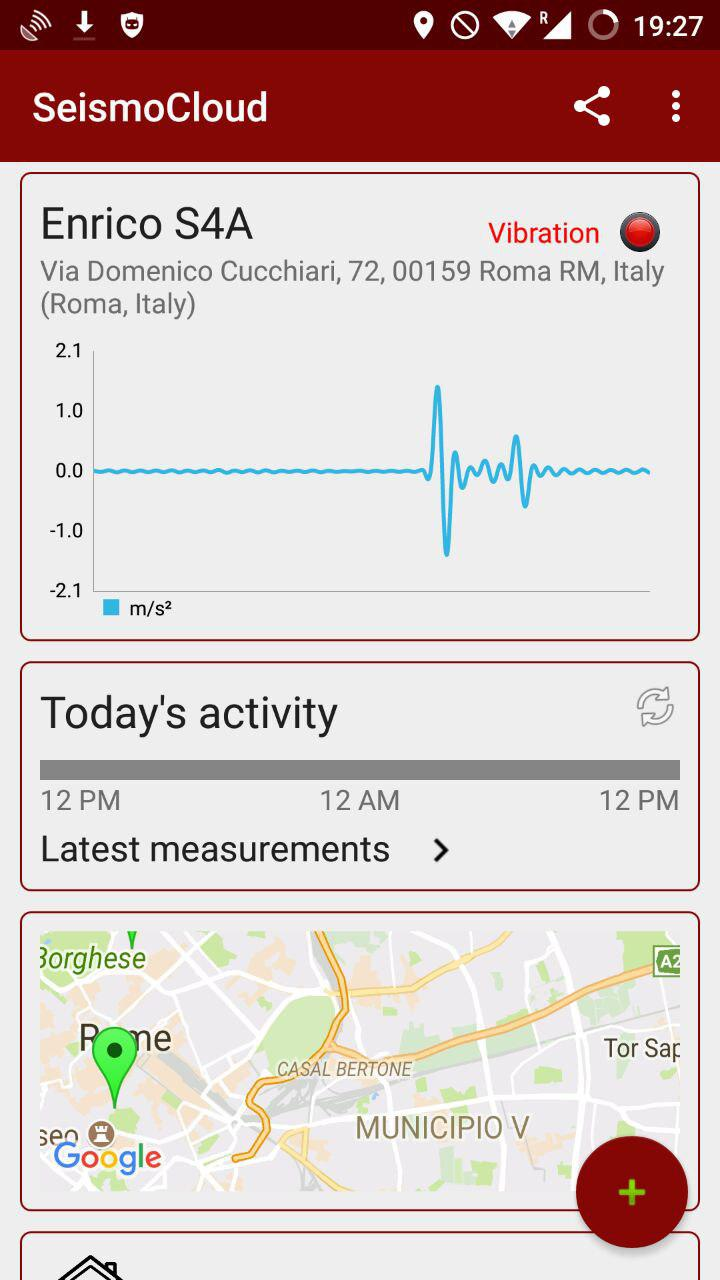
\includegraphics[scale=0.15]{app/main}
\end{center}
\end{frame}

\section{Ottimizzazione energetica}

\begin{frame}[c]{Contesti di attivazione (del servizio in background)}
Un \textbf{contesto di attivazione} è un insieme di variabili che, per opportuni valori, consentono al servizio di attivarsi.

\vspace{0.5cm}
In \textbf{SeismoCloud}, il contesto è definito come:
\vspace{0.2cm}
\begin{itemize}
  \item Rotazione/posizione del telefono
  \item Presenza o meno della localizzazione (GPS)
  \item Presenza o meno di uno spostamento (geografico)
  \item Presenza o meno della rete Internet
  \item Capacità rimanente batteria
\end{itemize}
\end{frame}

\begin{frame}[c]{Contesti di attivazione: diagramma di stato}
%\begin{center}
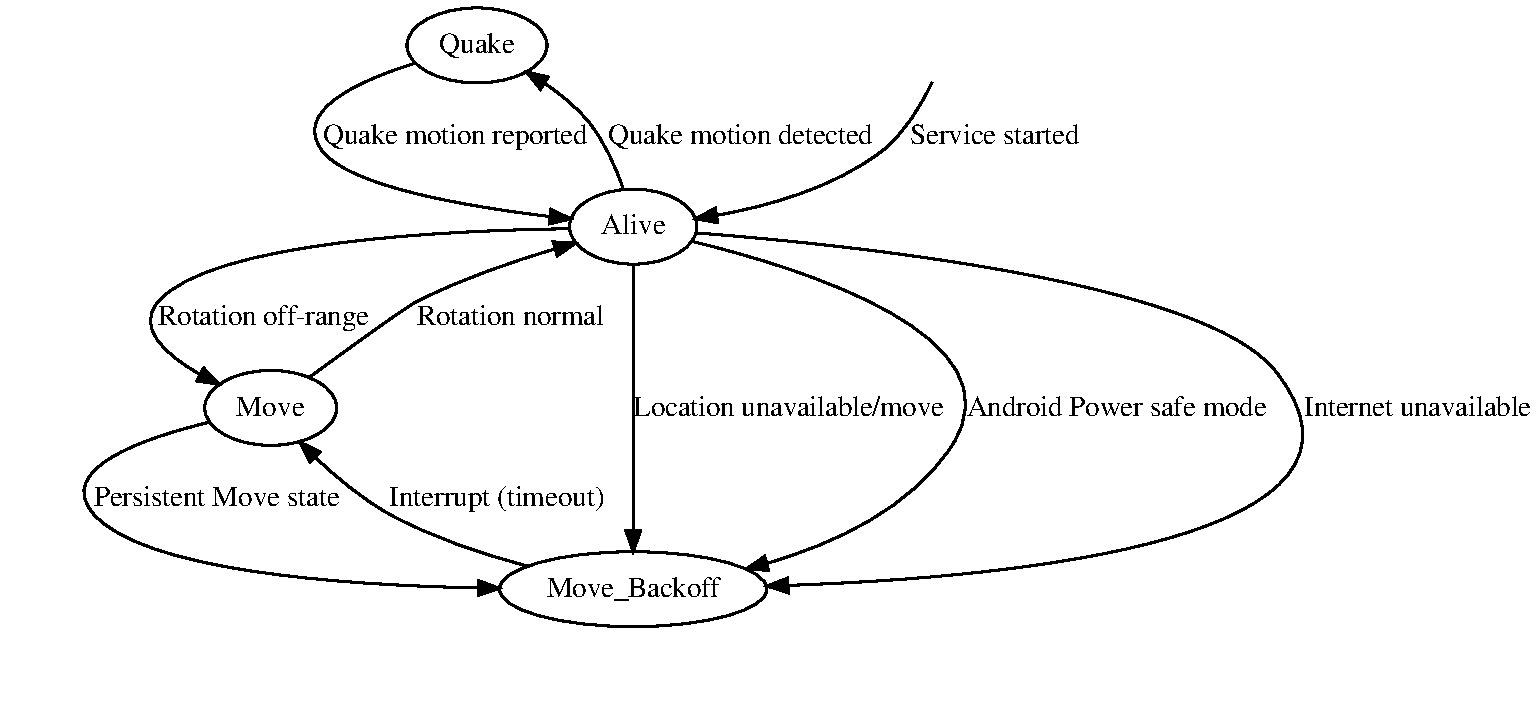
\includegraphics[scale=0.47]{StateMachine3}
%\end{center}
\end{frame}

\begin{frame}[c]{Contesti di attivazione: risultati}

\begin{center}
\begin{table}[h]
\begin{tabular}{llll}
& \textbf{Algoritmo originale} & \textbf{Algoritmo ottimizzato} &  \\
Servizio attivo   & 18h 24m & 6h 36m & \\
Servizio inattivo & mai     & 11h 48m & \\
Telefono spento   & 5h 36m  & 5h 36m &
\end{tabular}
\caption{Tempo di utilizzo delle risorse (media giornaliera)}
\end{table}
\end{center}

\end{frame}

\begin{frame}[t]{Contesti di attivazione: risultati}

\begin{center}
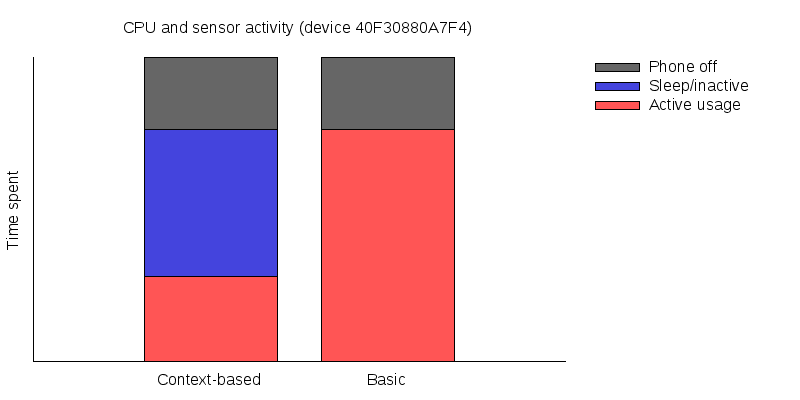
\includegraphics[width=\textwidth]{database/usageplot}
\end{center}

\end{frame}

\begin{frame}[c]{I sensori}

La app \textbf{SeismoCloud}, per effettuare la rilevazione, inizialmente utilizzava solo l'\textit{accelerometro}.

\vspace{1cm}

Per l'implementazione dei contesti di attivazione, è necessario utilizzare anche un sensore per la rotazione.

\end{frame}

\begin{frame}[c]{I sensori: giroscopio e magnetometro}

\begin{itemize}
  \item Una prima implementazione prevedeva l'uso del \textbf{giroscopio}
  \item Successivamente, si è affiancato l'uso del \textbf{magnetometro} come alternativa per telefoni di fascia bassa
  \item Il periodo di sampling, per entrambi i sensori (\textit{accelerometro} e \textit{giroscopio/magnetometro}) era di $20ms$
\end{itemize}

\end{frame}

\begin{frame}[c]{I sensori: tentativi di ottimizzazione}

Una prima ottimizzazione prevedeva l'uso di due periodi di sampling differenti: \textbf{ALIVE\_FAST} e \textbf{ALIVE\_SLOW}

\vspace{0.5cm}

\begin{center}
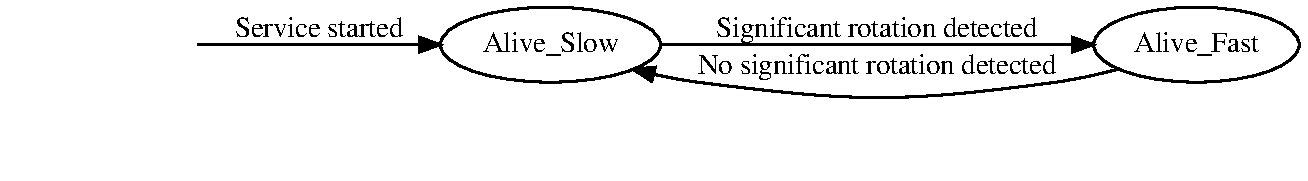
\includegraphics[width=\textwidth]{StateMachine4}
\end{center}

\vspace{0.5cm}

Tuttavia, lo studio ha evidenziato che il carico di CPU era equivalente, dunque questa ottimizzazione è stata abbadonata.

\end{frame}

\begin{frame}[c]{I sensori: il consumo}

Successivamente, uno studio sul consumo dei sensori ha evidenziato che il consumo del \textit{giroscopio} è di un ordine di grandezza superiore rispetto al consumo dell'\textit{accelerometro+magnetometro} (quasi sempre in un unico integrato).

\begin{table}[h]
\centering
\begin{tabular}{lllll}
& \textbf{In fase di misura} & \textbf{Stand-by} & \\
Accelerometro + Magnetometro \\
ADXL345 & $40 \mu A$ & $0.1 \mu A$ &  \\
Giroscopio \\
L3G4200D & $6.1mA$ & $0.2mA$ &
\end{tabular}
\end{table}

Dunque, è stato scelto di utilizzare sempre e solo \textbf{magnetometro} per la rotazione.

\end{frame}

\begin{frame}[c]{La curva di scarica}

Gli smartphones moderni hanno una autonomia limitata, dovuta anche (ma non solo) al numero di applicazioni in esecuzione.

\vspace{1cm}
Un modo aggressivo per limitare l'uso della batteria da parte di SeismoCloud è l'uso di una \textbf{curva di scarica}.

\end{frame}

\begin{frame}[c]{La curva di scarica: definizione}

\begin{equation}
\gamma = {85 \over 720}
\end{equation}

\begin{equation}
\lambda = \text{hour} * 60 + \text{minutes}
\end{equation}

\begin{equation}
    Threshold =
    \begin{cases}
        100 & \text{if hour} < 8\\
        15 & \text{if hour} > 20\\
        {100 - ((\lambda - 480) * \gamma)} & \text{otherwise.}
    \end{cases}
\end{equation}

Dove:
\begin{itemize}
\item $\gamma$: \textit{rate} di perdita capacità batteria per minuto (fascia 8-20)
\item $\lambda$: numero di minuti da mezzanotte del giorno attuale
\item $Threshold$: capacità della batteria (\%) prevista per l'orario attuale
\end{itemize}

\end{frame}

\begin{frame}[c]{La curva di scarica: valore atteso}

\begin{center}
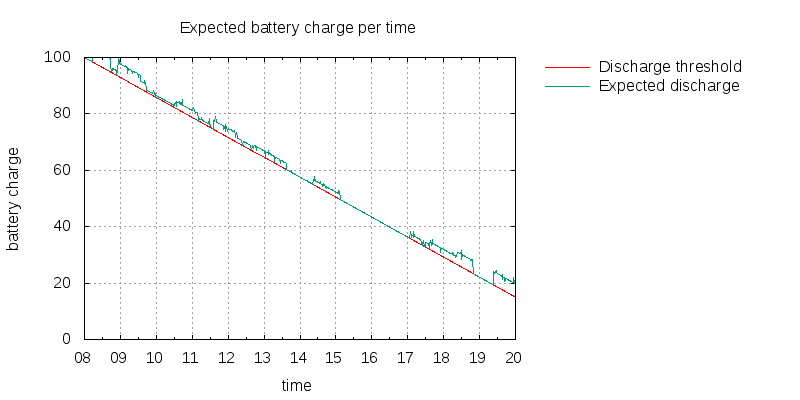
\includegraphics[width=\textwidth]{database/expectedplot}
\end{center}

\end{frame}

\begin{frame}[c]{La curva di scarica: risultati}

\begin{center}
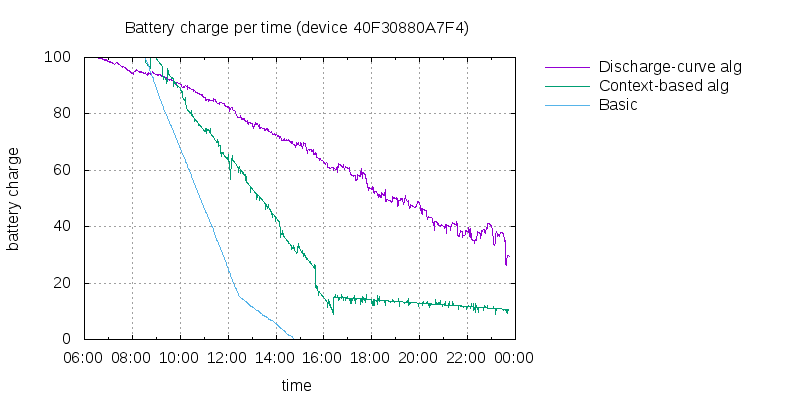
\includegraphics[width=\textwidth]{database/batteryplot}
\end{center}

\end{frame}

\section{Ottimizzazione della rete}

\begin{frame}[c]{Uso efficiente della rete}

Molti \textit{smartphones} sono connessi alla rete mediante una connessione tariffata \textit{a consumo}.
E' quindi importante rimuovere informazioni superflue dalla trasmissione.

\vspace{1cm}
Inoltre, un \textit{payload} alto nella trasmissione si traduce in un maggiore consumo di batteria.

\vspace{1cm}
E' quindi importante ottimizzare il protocollo di trasmissione allo scopo di ridurre il carico nella rete.

\end{frame}

\begin{frame}[c]{Message Queue Telemetry Transport}

\textbf{Message Queue Telemetry Transport} è un protocollo (standard ISO) di tipo \textit{publish-subscriber}, ottimizzato per operazioni in ambienti con memoria/rete limitati (ad esempio, per l'\textit{Internet of Things}).

\vspace{0.5cm}
Come altri protocolli \textit{publish-subscribe}, è basato sull'invio di messaggi da parte di \textit{publisher}, ruotati verso i sottoscrittori tramite \textit{topic} associati ai messaggio.

\vspace{0.5cm}
L'ottimizzazione, rispetto ad altri protocolli, è data dalla bassa complessità (e limitato numero di funzionalità) del protocollo.

\end{frame}

\begin{frame}[c]{MQTT in SeismoCloud}

Prima dell'ottimizzazione, il backend di SeismoCloud forniva solo API in HTTP.

\vspace{0.5cm}
Sebbene le API in HTTP siano ancora presenti (e utilizzate come \textit{fallback}), il backend è stato espanso per supportare MQTT.

\vspace{0.5cm}
L'utilizzo di MQTT, al posto di HTTP, permette alla \textit{App} di avere un basso \textit{footprint}, sia per quanto riguarda il codice in esecuzione, sia per quanto riguarda il traffico di rete.

\end{frame}

\begin{frame}[c]{MQTT vs HTTP}

\begin{table}[h]
\centering
\begin{tabular}{lll}
                    & \textbf{HTTP} & \textbf{MQTT} \\
\textbf{Overhead} & da 200 a 2048 bytes & 5-7 bytes \\
\textbf{Connessione} & 1 per richiesta & persistente \\
\textbf{Codifica header} & RFC 2822 & \textit{Type-Length-Value} \\
\textbf{Schema} & \textit{request/response} & \textit{publisher/subscriber} \\
\textbf{QoS} & - & 3 Livelli \\
\textbf{Dim. libreria} & Apache HTTP: 3 MB & Eclipse Paho: 14.6 KB \\
\end{tabular}
\end{table}

\end{frame}

\begin{frame}[c]{MQTT vs HTTP}

\begin{figure}[ht]
\centering
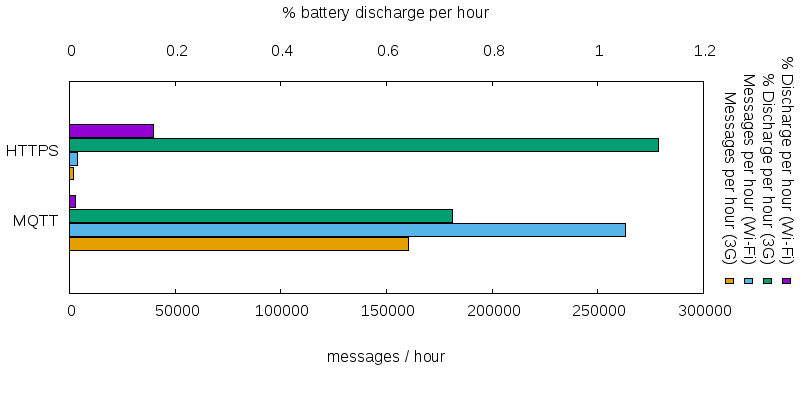
\includegraphics[width=\textwidth]{database/networkperformance0}
\end{figure}

\end{frame}

\section{Ottimizzazione in fase di sviluppo}

\begin{frame}[c,fragile]{Android Annotations: prima}

\begin{center}
    \begin{minipage}{\textwidth}

\begin{listing}[H]
\scriptsize
\begin{minted}[mathescape,
							 linenos,
							 numbersep=5pt,
							 gobble=0,
							 frame=lines,
							 framesep=2mm]{java}
public class SurveyActivity extends AppCompatActivity {
        private String param1;
        private String param2;

        @Override
        protected void onCreate(Bundle savedInstanceState) {
                super.onCreate(savedInstanceState);
                setContentView(R.layout.activity_survey);

                Intent in = getIntent();
                if (in == null) {
                        // Gestione dell'errore
                        this.finish();
                }
                param1 = in.getStringExtra("param1");
                param2 = in.getStringExtra("param2");
        }
        // Altro codice della activity
}
\end{minted}
\end{listing}

\end{minipage}
\end{center}

\end{frame}

\begin{frame}[c,fragile]{Android Annotations: dopo}

\begin{center}
\begin{minipage}{\textwidth}

\begin{listing}[H]
\scriptsize
\begin{minted}[mathescape,
							 linenos,
							 numbersep=5pt,
							 gobble=0,
							 frame=lines,
							 framesep=2mm]{java}
@EActivity(R.layout.activity_survey)
public class SurveyActivity extends AppCompatActivity {
        @Extra String param1;
        @Extra String param2;
        // Altro codice della activity
}
\end{minted}
\end{listing}

\end{minipage}

Grazie ad \textit{Android Annotations} il risparmio medio del codice è del $30\%$

\end{center}

\end{frame}


\begin{frame}[c]{LeakCanary}

\begin{figure}[ht]
\centering
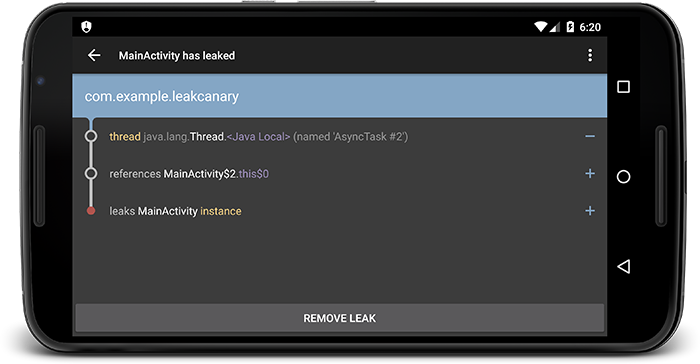
\includegraphics[width=0.8\textwidth]{dev/leakcanary}
\end{figure}

\end{frame}

\begin{frame}[c]{Application Crash Reports for Android}

\begin{figure}[ht]
\centering
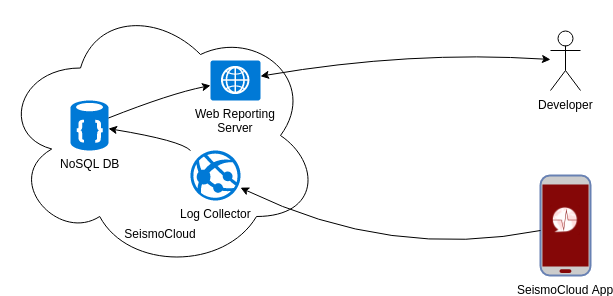
\includegraphics[width=0.9\textwidth]{dev/acracollector}
\end{figure}

\end{frame}

\begin{frame}[c]{Continuous integration}

Per mantenere sempre sotto osservazione il codice, è stata sviluppata una \textit{pipeline} per il processi di build utilizzando \textbf{SonarQube}, \textbf{Jenkins} e \textit{tool} specifici di Google per Android:

\vspace{0.5cm}
\begin{figure}[ht]
\centering
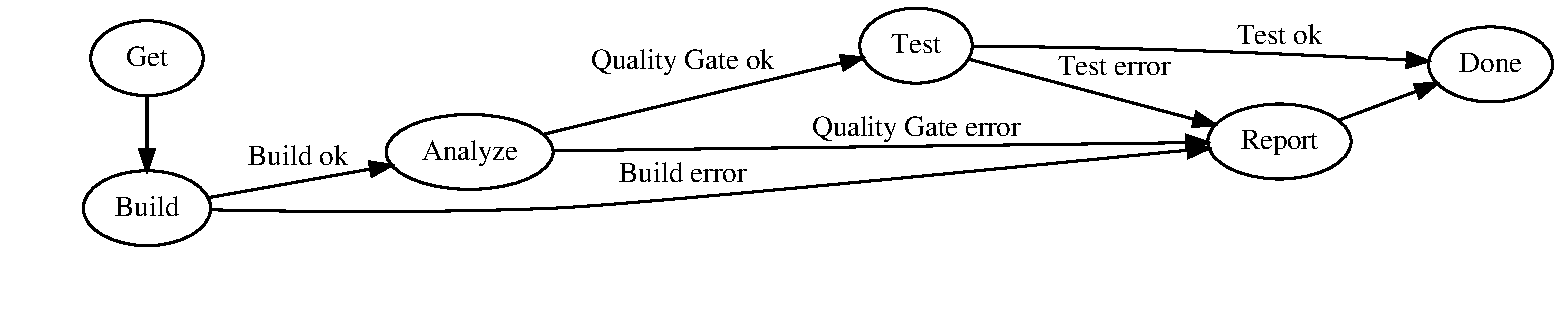
\includegraphics[width=\textwidth]{CIStateMachine}
\end{figure}

\end{frame}

\begin{frame}[c]{Continuous integration}

\begin{figure}[ht]
\centering
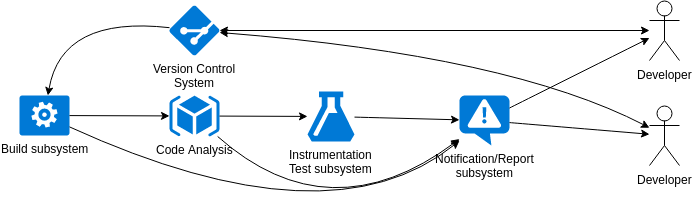
\includegraphics[width=\textwidth]{dev/ci}
\end{figure}

\end{frame}

\section{Sviluppi futuri}

\begin{frame}[c]{Sviluppi futuri}

\begin{enumerate}
	\item Sistema di spegnimento \textit{a zone geografiche}
	\item Utilizzo di sensori dedicati (se presenti)
	\item Porting del codice di pre-filtro in modo nativo (C/C++) per ottimizzazione energetica
	\item Tecniche avanzate per l'ottimizzazione del rilevamento della posizione geografica
\end{enumerate}

\end{frame}

\revslide{Grazie}
